\chapter{Participant Demographics}
\section{Overview}
This chapter provides all the data collected on my participants before any experiment was carried out. The purpose of this was to categorise participants into the Novice and Experienced groups. Data collected included generic demographics such as gender, age and highest level of education. More specific data surrounding the participants knowledge on gaming themes such there overall familiarity with games, how long they would play games for per week and what types of outlets they would use in order to play these games was also collected. 

\section{Pre-Experiment Questionnaire - General Demographics}
\subsection{Gender Demographics}
\begin{figure}[H]
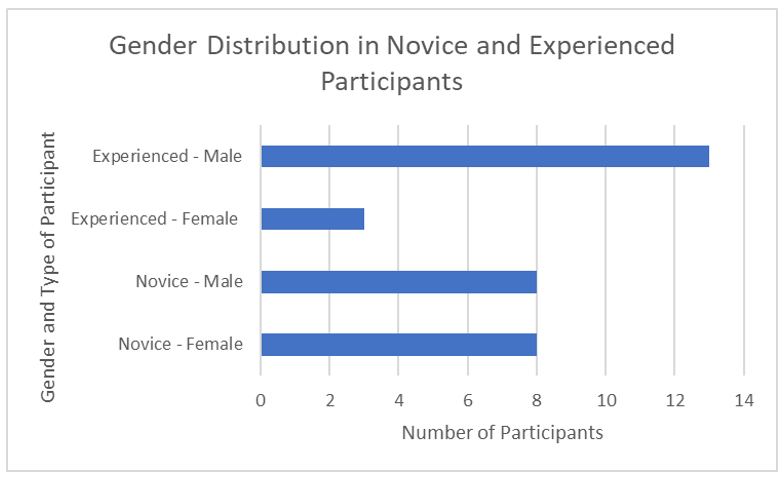
\includegraphics[width=\linewidth]{Screenshots/DemographicsQuestionaires/genderDistribution.png}
\label{GenderDistribution}
\caption{Gender Distribution of Novice and Experienced Participants}
\end{figure}

This graph displays the numbers of female and male participants in both Novice and Experienced categories. On first glance the Novice group is balanced with eight males and eight female participants thus having a 50/50\% split. However male and female participants within the Experienced category are unbalanced with 13 male (81.25\%) to only three female (18.75\%) participants and as such can be considered one limitation in this study, to be discussed later in Chapter 8, Conclusion.  


\subsection{Novice Demographics}
\begin{figure}[H]
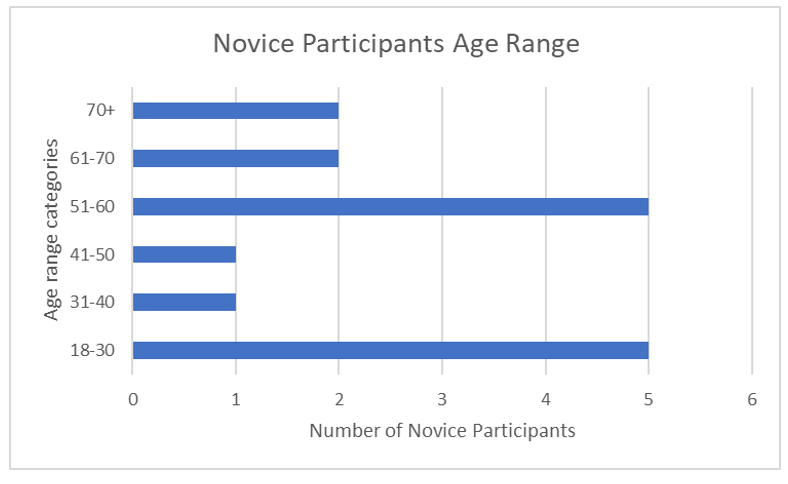
\includegraphics[width=\linewidth]{Screenshots/DemographicsQuestionaires/noviceAgeRange.png}
\label{NoviceAges}
\caption{Novice Age Range}
\end{figure}

This graph shows the distribution of age groups within the Novice category. The two largest groups were participants aged between 18-30 and and 51-60, with each category holding five participants or 31.25\% of the total group population. 61-70 and 70+ categories held two participants each, accounting for 12.5\% of the population each. Lastly 31-40 and 41-50 categories held one participant each thus accounting for 6.25\% for each category in the total sample of participants totalling 16 overall. 

\begin{figure}[H]
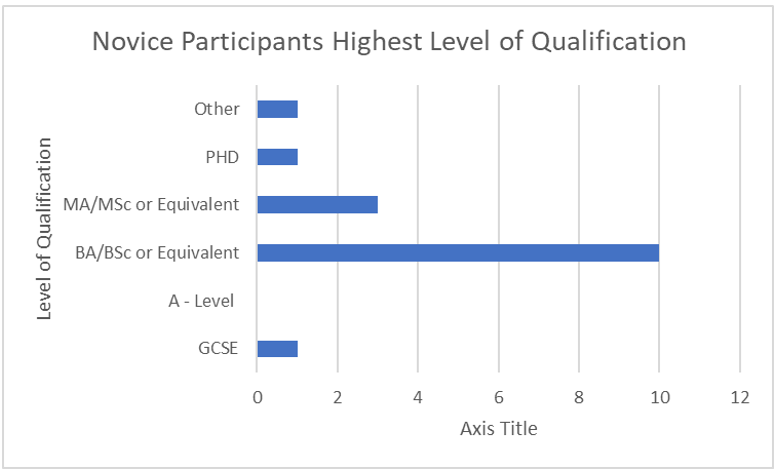
\includegraphics[width=\linewidth]{Screenshots/DemographicsQuestionaires/noviceEducation.png}
\label{NoviceQualifications}
\caption{Novice Participants Highest Level of Qualification}
\end{figure}

There are several levels of qualification that were answered by the novice participants. 10 (62.5\%) of participants holding a BA/BSc or equivalent qualification. Three participants (18.75\%) held an MA/MSc or equivalent. The remaining groups held one participant each (6.25\%) with the exception of the A-Level category with no participants answering that as their highest level of qualification.

\subsection{Experienced Demographics}
\begin{figure}[H]
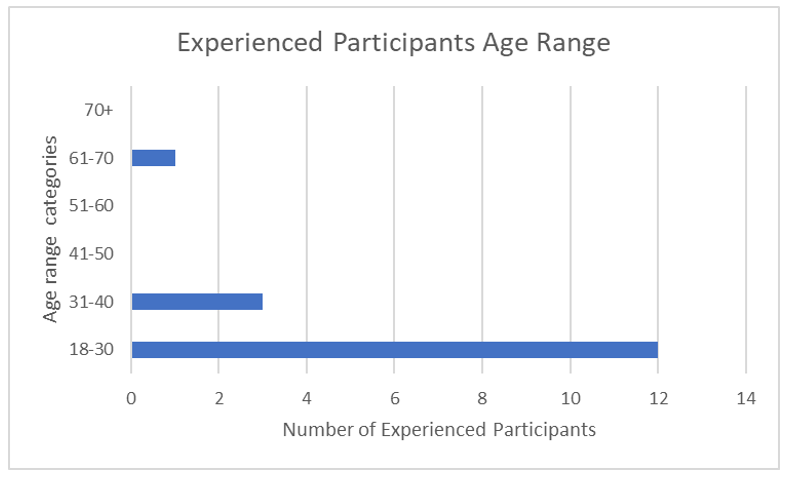
\includegraphics[width=\linewidth]{Screenshots/DemographicsQuestionaires/experiencedAgeRange.png}
\label{ExperiencedAges}
\caption{Experienced Participants Age Range}
\end{figure}

The age range of participants within the experienced category shares a similar issue to that of gender distribution within this category. This is because 12 of the 16 participants were aged in the 18-30 age range thus accounting for 75\% of the experienced population sample. Therefore only three participants were aged between 31-40 and only one participant aged in 61-70 category. However this distribution is in keeping with general trends within the gaming industry with those aged between 18-30 being one of the most popular users of games services, extending up to the age of 40 according to 2017 global statistics \citep{gamersChristinaGough2017}. 

\begin{figure}[H]
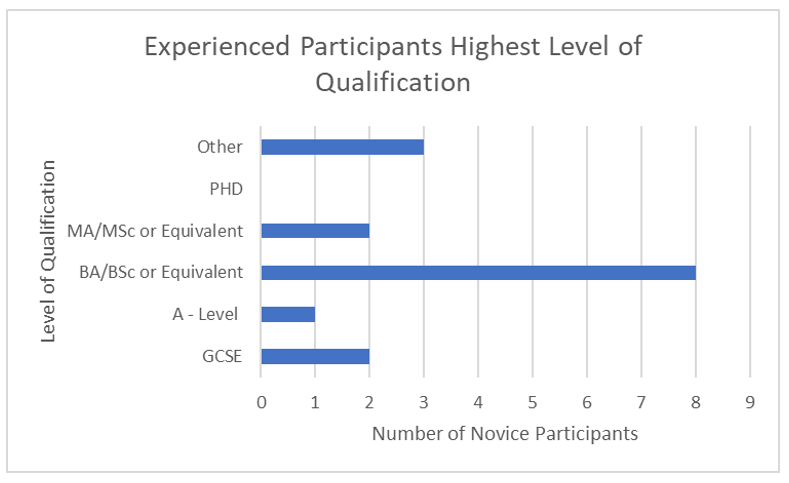
\includegraphics[width=\linewidth]{Screenshots/DemographicsQuestionaires/experiencedEducation.png}
\label{ExperiencedQualifications}
\caption{Experienced Participants Highest Level of Qualification}
\end{figure}

Similarly to that of the Novice participants, there was a wide range of levels of education, with the same majority of participants holding at least a BA/BSc or equivalent qualification. However those who held a BA/BSc or equivalent qualification only totalled eight or 50\% of the sample population, as compared with 12 or 75\% of the Novice sample population. Three (18.75\%) participants held qualifications that did not fit into other categories, two holding (12.5\%) MA/MSc or equivalent, a further two (12.5\%) with at least GCSE and one participant with A-level qualifications. 

\section{Novice Pre-Experiment Questionnaire Gaming Queries}
The following section details some key information that I asked my Novice participants before and after there involvement in my study, with specific queries relating to their knowledge on gaming services and their thoughts on the \gls{ta} process during there testing session.

\subsection{Gaming Familiarity}
\begin{figure}[H]
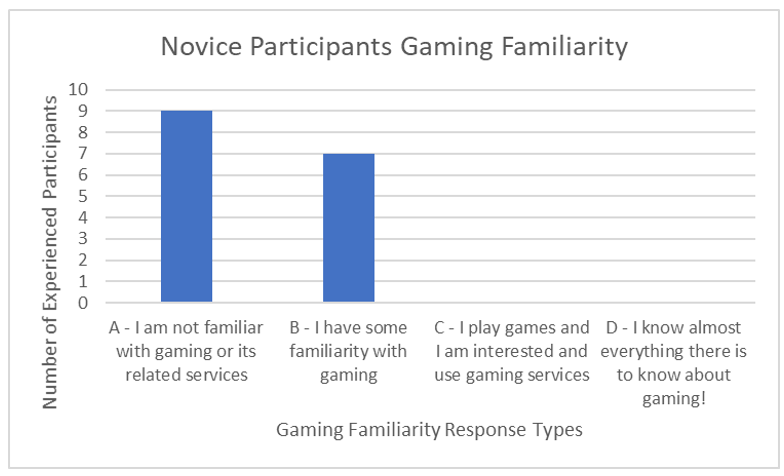
\includegraphics[width=\linewidth]{Screenshots/DemographicsQuestionaires/noviceQuestionaireData/noviceParticipantsGamingFamiliarity.png}
\label{NoviceGamingFamiliarity}
\caption{Novice Participant's Familiarity with Gaming}
\end{figure}

This graph details how my Novice participants responded to the question asking them how familiar they were with gaming concepts. This could be personally through their own usage, or vicariously such as with a sibling or child's interest in gaming. Unsurprisingly all my novices responded with A or B which means that their overall knowledge in gaming is limited, as anticipated when formulating this research. Out of 16 participants, nine or 56.25\% responding that they were not familiar with gaming at all, with the remaining seven or 43.75\% of participants answering B, thus holding some limited knowledge within gaming. 

\subsection{Gaming Devices Ownership}
\begin{figure}[H]
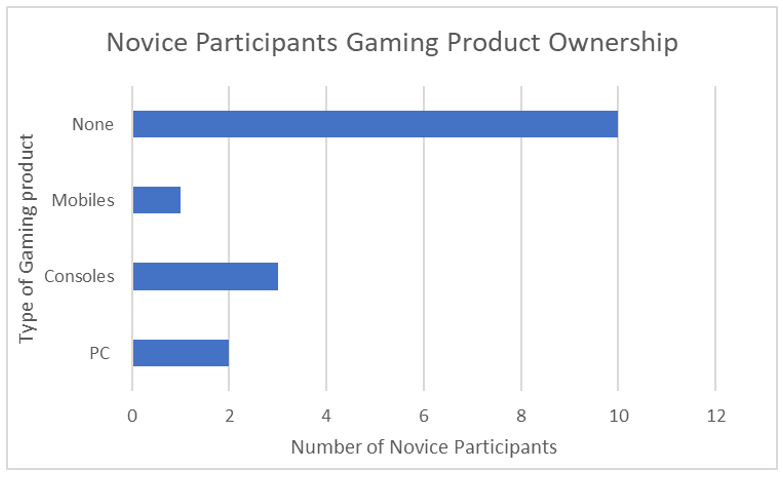
\includegraphics[width=\linewidth]{Screenshots/DemographicsQuestionaires/noviceQuestionaireData/noviceGamingOwnership.png}
\label{NoviceGamingOwnership}
\caption{Novice Gaming Product Ownership and Usage}
\end{figure}

After asking the Novice participants for their overall gaming knowledge, a question regarding which devices they owned and used was also asked. The majority of the 16 participants answered that they owned no dedicated gaming devices and devices capable being used for gaming were not used for that purpose, totalling ten participants. There were six participants who were in the sample minority. Three participants (18.75\%) answered that they owned Consoles such as a Sony PlayStation 4, two participants (12.5\%) owning a PC used for gaming purposes, and one novice participant (6.25\%) who used their mobile phone to casual play games on. 

\subsection{Time Spent Gaming}
\begin{figure}[H]
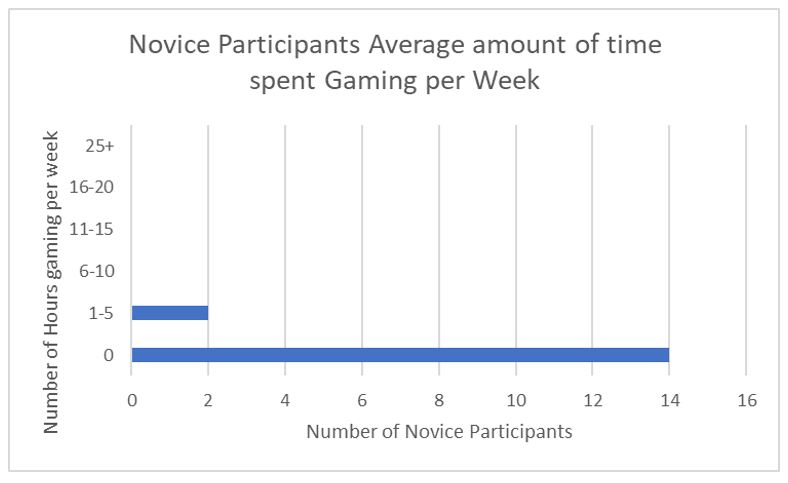
\includegraphics[width=\linewidth]{Screenshots/DemographicsQuestionaires/noviceQuestionaireData/noviceTimeSpentGaming.png}
\label{NoviceTimeGaming}
\caption{Novice Participants average Time Spent Gaming per week}
\end{figure}

This data is a further expansion to the data collected in Figure 4.7. As expected the majority of participants answered that they did not spend any time per week gaming on any devices. Only two participants (12.5\%) answered that they played for a brief time period of 1-5 hours a week. Thus confirming that my participants were complete novices to gaming, or at most extremely casual players of games. 

\section{Experienced Pre-Experiment Questionnaire Gaming Queries}
The following section details some key information that experienced participants were asked, before and after their involvement in my study with specific queries relating to their knowledge on gaming services and their thoughts on the \gls{ta} process during there testing session.

\subsection{Gaming Familiarity}
\begin{figure}[H]
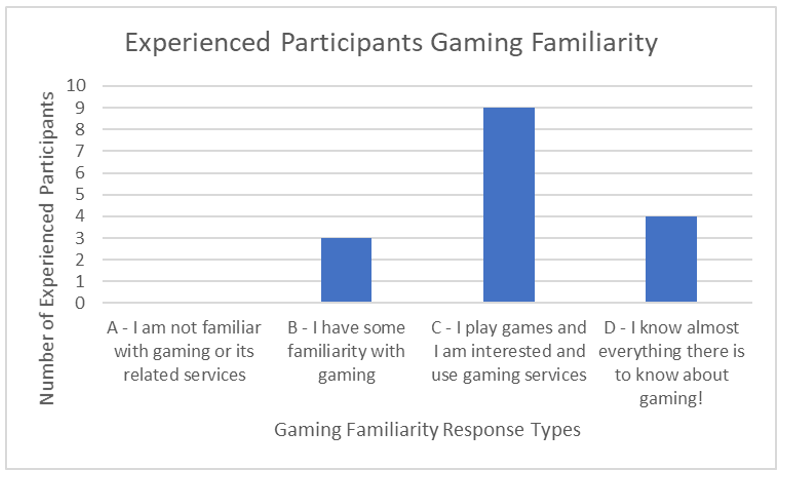
\includegraphics[width=\linewidth]{Screenshots/DemographicsQuestionaires/experiencedQuestionaireData/experiencedParticipantsGamingFamiliarity.png}
\label{ExperiencedGamingFamiliarity}
\caption{Experienced Participants Familiarity with Gaming}
\end{figure}

This figure shows the response from my experienced participants in relation to gaming familiarity. Nine participants (56.25\%) responded with option C, 4 (25\%) with option D, and three (18.75\%) with option B. No participants in the experienced category answered with response A, which was expected as if they had, they would have placed them into the Novice category.

\subsection{Gaming Devices Ownership}
\begin{figure}[H]
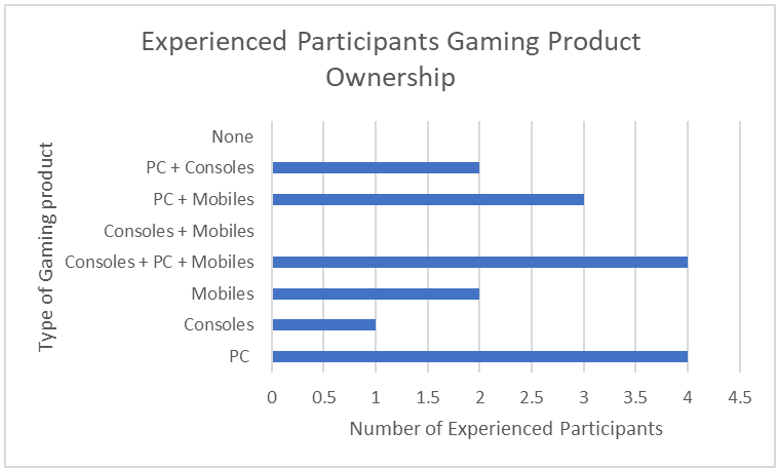
\includegraphics[width=\linewidth]{Screenshots/DemographicsQuestionaires/experiencedQuestionaireData/experiencedGamingOwnership.png}
\label{ExperiencedGamingOwnership}
\caption{Experienced Participants Gaming Product Ownership and Usage}
\end{figure}

This figure is more diverse then that of the Novice counterpart (see Figure \ref{NoviceGamingOwnership}). Experienced participant's gave a series of answers including that of hybrid answers which included two or more options for which outlets they use for gaming. The most common outlets were PC and PC,Console and Mobile use, with four participants in each category accounting for 50\% of the sample population together. Three participants (18.75\%) answered that they used PC and Mobiles, two answered that they owned only mobiles and another two answered that they owned a PC and a gaming console accounting for a further 25\% of the sample population. Only one participant answered that they only owned a gaming console. Interestingly no participants answered that they owned consoles and mobiles together for gaming purposes. Therefore this sample has a wide range of participants with different gaming devices, and therefore expectations on how they would work, especially regarding UI/UX elements.

\subsection{Time Spent Gaming}
\begin{figure}[H]
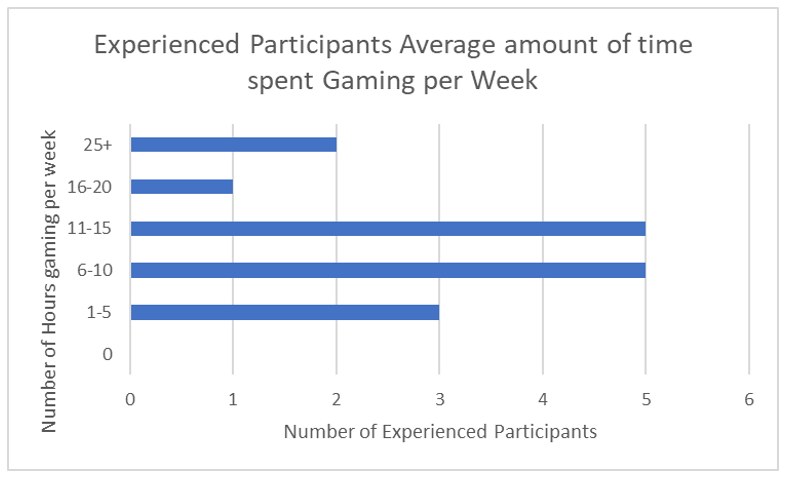
\includegraphics[width=\linewidth]{Screenshots/DemographicsQuestionaires/experiencedQuestionaireData/experiencedTimeSpentGaming.png}
\label{ExperiencedGamingTime}
\caption{Experienced Participants average Time Spent Gaming per week}
\end{figure}

This figure shows that the experienced participants have a varied amount of time spent gaming in an average week of there's, with five participants in 6-10 and 11-15 hours each, thus accounting for 62.5\% of the population. Three participants answered that they played between 1-5 hours a week, which two of the novice participants also answered. However due to other factors such as gaming familiarity and device ownership, these participants are still categorised as experienced participants, despite the similarities to those Novice participants who answered the same way with this metric. Two participants answered that they played over 25 hours a week and as such are considered the most experienced participants. One participant answered that they played 16-20 hours a week and thus they were another highly experienced gaming user. Overall, my experienced category was quite diverse regarding this specific metric.


\section{Post Experiment Questionnaire}
\subsection{Novice Participant Responses}
\begin{figure}[H]
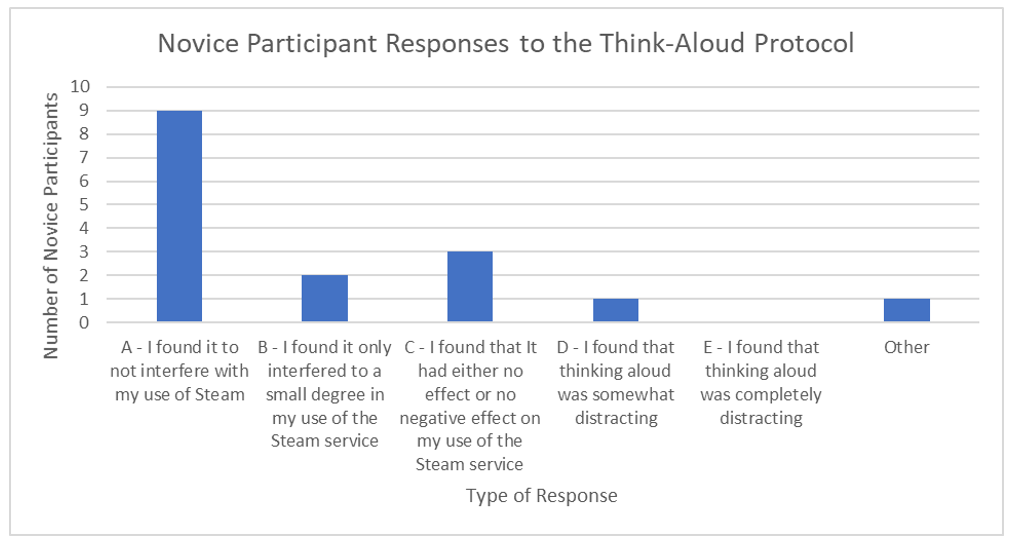
\includegraphics[width=\linewidth]{Screenshots/DemographicsQuestionaires/noviceQuestionaireData/noviceTAP.png}
\label{NoviceTAP}
\caption{Novice Participants responses to the Think-Aloud Protocol}
\end{figure}

This graph shows the distribution of answers given by Novice participants following the experiment regarding the \gls{ta} Protocol. Participants were asked to rate there thoughts on the \gls{ta} methodology, in terms of how they thought it effected there ability to complete the test. For instance, did Thinking aloud distract Novices in there attempts at using the program? This graph shows that not to be the case for the majority of participants. Nine participants (56.25\%) answered that with response A and thought that Thinking allowed did not distract them whilst using the Steam service. A further two did respond that Thinking aloud did interfere with there use of Steam to a minor degree. However one participant found that concurrently Thinking aloud was of somewhat detrimental to the testing process, elaborating that they could not really talk and use the program at the same time. Three participants found the \gls{ta} Protocol has no effect on there use of Steam. Interestingly the last participant found that by thinking aloud it actually helped them use the Steam program, this is indicated by the ``Other" response. 

\begin{figure}[H]
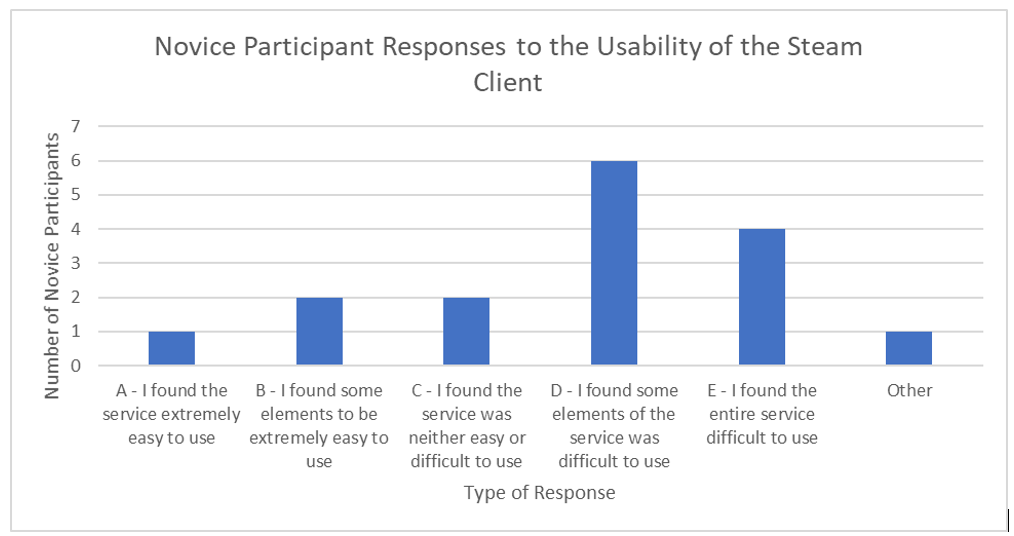
\includegraphics[width=\linewidth]{Screenshots/DemographicsQuestionaires/noviceQuestionaireData/noviceSteamClient.png}
\label{NoviceSteamUsability}
\caption{Novice Participants responses to the Usability of the Steam Service}
\end{figure}

When asked what there thoughts were on the Steam interface most Novice participants responded that they found some of the service difficult to use. This response was given by six participants with a further four saying that the entirety of Steam was difficult to use. A further participant gave the response ``D/E" as indicated by the ``Other" category. This is somewhat perplexing, but still the participant gave Steam a negative usability rating. Thus, category D, E and the hybridised answer accounted for 11 participants or 68.75\% of the sample population. Conversely two novices found that some elements were extremely easy to use, with only one novice saying that they found the entire service easy to use, therefore making up 18.75\% of the total novice sample. The last two participants gave a neutral rating to the usability of Steam regarding the six tasks they had attempted and made up the final 12.5\% of the novice sample population.

\subsection{Experienced Participant Responses}
\begin{figure}[H]
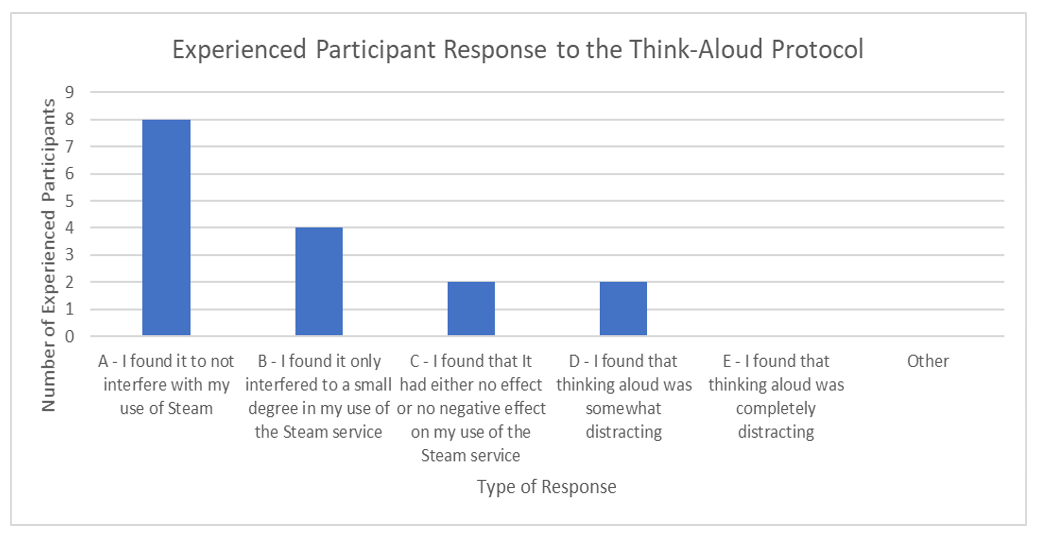
\includegraphics[width=\linewidth]{Screenshots/DemographicsQuestionaires/experiencedQuestionaireData/experiencedTAP.png}
\label{ExperiencedTAP}
\caption{Experienced Participants responses to the Think-Aloud Protocol}
\end{figure}

When asked for their thoughts on the \gls{ta} methodology, most experienced participants reacted similarly to that of Novices, with the majority finding that concurrently thinking aloud did not impact their usage of the Steam service. Eight participants answered that Thinking aloud to not interfere with Steam, with a further four saying that it only interfered there use of the program to a small degree, thus account for 75\% of participants. Only two participants (12.5\%) answered that Thinking-aloud was distracting during the experiment. The remaining two participants (12.5\%) answered that Thinking aloud did not impact them in any way at all. 

\begin{figure}[H]
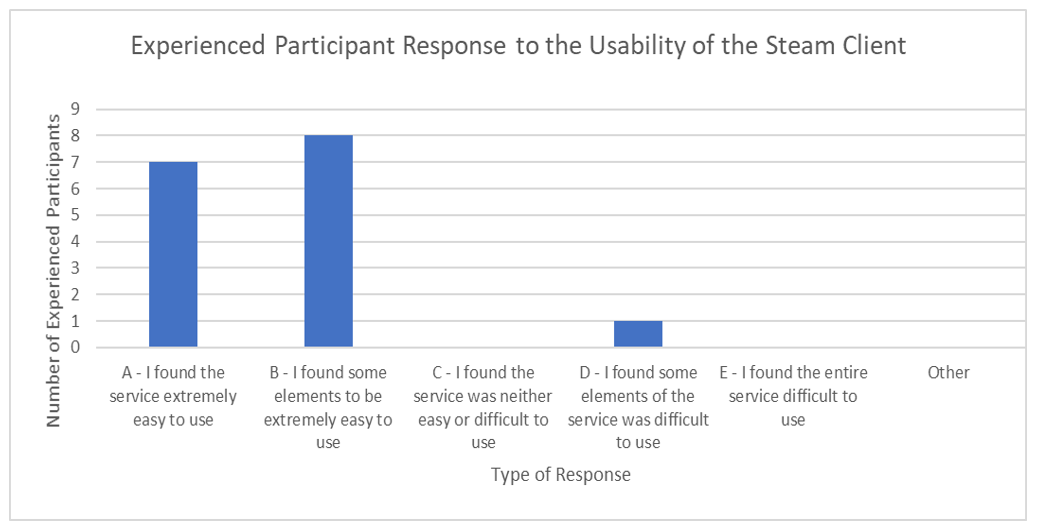
\includegraphics[width=\linewidth]{Screenshots/DemographicsQuestionaires/experiencedQuestionaireData/experiencedSteamClient.png}
\label{ExperiencedSteamUsability}
\caption{Experienced Participants responses to the Usability of the Steam Service}
\end{figure}

Lastly, as expected the majority of the experienced participants responded positively when asked about the usability of the Steam service. Only 1 participant answered that they found the service to be somewhat difficult to use, especially with regards to Task C and D. The remaining 15 participants however reacted positively, with 7 participants saying that the service was extremely easy to use, and the remaining 8 saying that some elements were extremely easy. Thus saying that for the most part Steam seemed to be quite an innovative service.
